\section{A hierarchy defined by finite local rules}\label{sec:finite-rules}

Our objective is a finite presentation with two simultaneous
properties: clean encodings preserve nonzero words from the next level,
and sufficiently long nonzero words admit the token decomposition used
for matrix cancellation. The two properties require different arguments.
We must control every sequence of replacements starting from an encoded
word, and we must also analyze words containing control states that no
such sequence ever reaches.

We use presentations of associative algebras by words.  An elementary
replacement is a relation $v=v'$ between nonempty words of the same
length; it may be used in either direction inside a word.  An elementary
zero declaration is a relation $v=0$, with $v$ nonempty.  The lengths of
these relations mean the lengths of $v$ and $v'$, not their degrees as
binomials.

\begin{lemma}\label{fr:basis}
For a presentation of this kind over a field $K$, the nonzero
replacement classes of words form a $K$-basis of the algebra.  A class is
zero precisely when one of its words contains an elementary
zero-declared substring.  The empty word is one of the surviving
classes, and the algebra is graded by word length.
\end{lemma}

\begin{proof}
Make a graph whose vertices are words, including the empty word, and
whose edges are elementary replacements in arbitrary contexts.  The
ideal generated by the binomial relations is the span of the differences
between vertices in a common connected component.  Quotienting by it
leaves one basis vector per component.  The ideal generated in this
quotient by the zero declarations is the span of the components
containing a word with a declared zero substring.  No edge changes
length, and no zero declaration involves the empty word.
\end{proof}

Here and throughout this Section, the parameter $h$ is a positive
integer and $q_h=2^h$.  Bounds asserted for sufficiently large $h$ are
uniform along the sequence of parameters used in the following
Proposition.  A field is not part of the rule table: the same word
relations are used over every field. Besides its color, a palette
letter has a finite tuple of auxiliary data, called its non-color
fields. These include two control tracks, one checking colors and one
verifying an encoded rule.
Each track designates whether a head is present at a cell; the rule
construction below specifies these head flags.

\begin{proposition}\label{prop:hierarchy}
There are absolute positive integers $c,k$, with $c=10000$ and $k=10$
permitted, with the following property.  Fix an integer $D\geq2$.
There is an integer $h_0$ and, for every
\[
 h\in\{h_0,h_0D,h_0D^2,\ldots\},
\]
a finite alphabet $\Sigma_h$, of cardinality at most $2^{ch}$, and a
finite table of elementary replacements and zero declarations of
length at most $k$.  Write $A_h(K)$ for the resulting unital
associative algebra over a field $K$, and write $[w]$ for the image of a
word.  These tables have the following three properties.
\begin{enumerate}
\item\label{fr:prop-encoding}
There is a fixed-length substitution
$E_h:\Sigma_{Dh}\longrightarrow\Sigma_h^{L_h}$, where
$L_h=2q_h+1$.  Every elementary relation or zero declaration at
parameter $Dh$ is a consequence of the relations at parameter $h$
after substitution.  Thus $E_h$ induces a unital algebra homomorphism
$A_{Dh}(K)\longrightarrow A_h(K)$.  If a word $w$ is nonzero at
parameter $Dh$, then $E_h(w)$ is nonzero at parameter $h$.
There is a nonzero one-letter word at every parameter.
\item\label{fr:prop-tokens}
A subset of $\Sigma_h$ specifies cuts immediately before its letters.
There are a bound $B_h$ and a finite list $\mathcal T_h$ of tokens such
that every sufficiently long nonzero word has a unique decomposition
\[
 p\,t_1\cdots t_r\,s,
 \qquad t_i\in\mathcal T_h,\qquad |p|,|s|\leq B_h.
\]
Here $p$ is the part before its first cut, $s$ is the part from its last
cut, and the $t_i$ are exactly the intervals between consecutive cuts.
Cuts are counted only when their following letter occurs in the word.
Each token starts with a cut letter and has no other cut letter.
For each $t\in\mathcal T_h$ there is a nonempty word $u_t$ over
$\Sigma_{Dh}$ such that
\[
 1\leq |u_t|\leq k,
 \qquad |t|=L_h|u_t|,
 \qquad [t]=[E_h(u_t)].
\]
The equalities can be effected by replacements supported inside the
token.  No assertion is made that arbitrary concatenations of tokens
are nonzero.
\item\label{fr:prop-runs}
Some letters are designated palette letters and have a color in a set
of $q_h$ colors.  An eligible run consists of consecutive palette
letters with a common tuple of non-color fields and with neither of
the two control-track head flags set.  Every adjacent transposition
within such a run is an elementary replacement of the whole letters.
Every eligible run in a nonzero word has pairwise distinct colors.
Every sufficiently long nonzero word contains an eligible run of
length at least $q_h/100$.  Eligibility and the endpoints of maximal
eligible runs depend only on the non-color fields.
\end{enumerate}
The integer $D$ is chosen before the program fixed point used to
define the tables; $h_0$ is chosen afterward.  The constants $c,k$ do
not depend on $D$.
\end{proposition}

We give the rule tables and then prove their properties.  Giving a
finite predicate for table membership specifies an ordinary finite
presentation: enumerate all words of length at most $k$ over the
finite alphabet and retain exactly the declared entries.  No relation
at another parameter is itself included in the table at $h$.

\subsection{The alphabet and its encoded blocks}
\label{fr:formats}

Take $\Sigma_h$ to be the set of all bit strings of length $ch$.
The following named
fields are placed in fixed disjoint slots; unused bits must be zero.
For definiteness, reserve 32 integer slots of width $2h$ and 512
individual flag slots, and fill the remaining positions with zero.
Only a fixed number of these slots will be used.  Thus $c=10000$
suffices, including at $h=1$.  Integers have ordinary binary encodings;
zero-based encodings may be used for intervals beginning at 1.  A
letter with an out-of-range field or an unlisted combination of tags
is declared zero, but remains a letter of $\Sigma_h$. Once $D$ is fixed,
the allowable ranges and the
assignment of named fields are given by the procedures below.

The structural type of a letter is $C(p)$, $P(a)$, or $S$, where
$1\leq p\leq q_h$ and $1\leq a\leq q_h$.  The number $p$ is a core
position and $a$ is a palette color.  The only allowed structural
adjacencies are
\begin{equation}\label{fr:structural-pairs}
 C(p)C(p+1),\quad C(q_h)P(a),\quad P(a)P(b),\quad P(a)S,
 \quad SC(1).
\end{equation}
The first adjacency requires $p<q_h$.  Every other structural pair is
declared zero.  Thus a complete block has $q_h$ core cells, a nonempty
palette, and a stop cell.  Missing neighbors at the ends of the whole
word impose no structural test.

Each letter also has a transaction control track, and each palette cell
has an independent palette-checker track. Each track has a distinguished
idle state; its nonidle states will be listed below. A core cell whose
transaction track is idle has a data bit if $p\leq cDh$ and has no data
otherwise. The first $cDh$ data bits of a complete idle block therefore
encode one letter of $\Sigma_{Dh}$, whether or not that letter satisfies
the format restrictions at parameter $Dh$. Palette and stop cells have
no data payload. These are unary format requirements. We take $h$
large enough that $cDh\leq q_h$.

A \emph{clean block} has both tracks idle and has each palette color
exactly once. It is \emph{canonical} when those colors occur in increasing
order. For $a\in\Sigma_{Dh}$, let $E_h(a)$ be the canonical block whose
core data are the $cDh$ bits of $a$, and extend $E_h$ to words by
concatenation. Its block length is $L_h=2q_h+1$.
Figure~\ref{fr:block-figure} shows this chosen encoding. Structural
syntax alone still allows any nonempty palette: its length and colors
will be forced only by the nonzero-word arguments.
\begin{figure}[htbp]
\centering
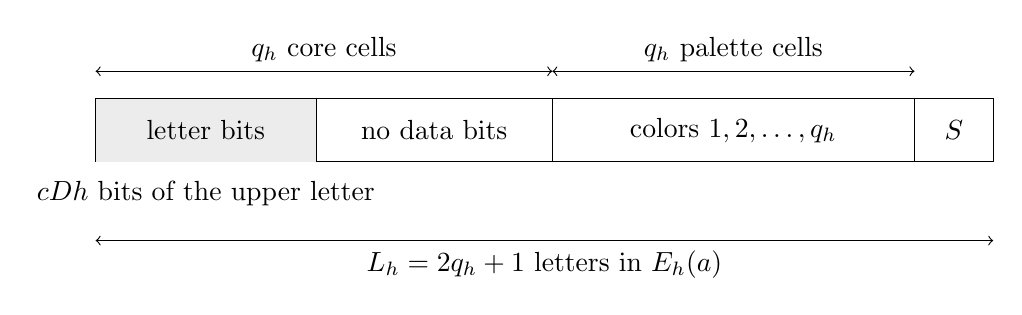
\begin{tikzpicture}[x=1cm,y=1cm]
 \draw (0,0) rectangle (11.4,0.8);
 \fill[gray!15] (0,0) rectangle (2.8,0.8);
 \draw (2.8,0)--(2.8,0.8);
 \draw (5.8,0)--(5.8,0.8);
 \draw (10.4,0)--(10.4,0.8);
 \node at (1.4,0.4) {letter bits};
 \node at (4.3,0.4) {no data bits};
 \node at (8.1,0.4) {colors $1,2,\ldots,q_h$};
 \node at (10.9,0.4) {$S$};
 \draw[<->] (0,1.15)--(5.8,1.15);
 \node[above] at (2.9,1.15) {$q_h$ core cells};
 \draw[<->] (5.8,1.15)--(10.4,1.15);
 \node[above] at (8.1,1.15) {$q_h$ palette cells};
 \node[below,align=center] at (1.4,-0.12) {$cDh$ bits of the upper letter};
 \draw[<->] (0,-1.0)--(11.4,-1.0);
 \node[below] at (5.7,-1.0) {$L_h=2q_h+1$ letters in $E_h(a)$};
\end{tikzpicture}
\caption{A canonical block encoding one letter $a\in\Sigma_{Dh}$.
The core carries its $cDh$ data bits, the palette contains each color
once in increasing order, and the stop cell closes the block. Both
control tracks are idle. The widths are schematic; the data positions
fit inside the core by the choice of $h_0$.}
\label{fr:block-figure}
\end{figure}


The replacements will carry out a proposed upper-level relation inside
one or more complete blocks. They temporarily acquire the cells of those
blocks, keeping the present data and a proposed replacement in separate
slots. The verifier checks a certificate for the proposed relation before
the replacement can become the represented data. We first specify the
control fields that keep this operation confined to its own cells.

\subsection{Control tracks and admissible neighboring pairs}

The palette-checker track has states
\[
 I,\qquad A_x,\qquad H_x\qquad(1\leq x\leq q_h),
\]
meaning idle, passed while seeking $x$, and the checker head seeking
$x$. The checker-head flag is set exactly in state $H_x$.
Within a palette the allowed adjacent checker-state pairs are
\[
 (I,I),\qquad (A_x,A_x),\qquad (A_x,H_x),
 \qquad (H_x,I).
\label{fr:checker-pairs}
\]
There is no restriction on the first palette state except its format;
the last palette state must be $I$ or $H_x$.  These are pair tests at
$C(q_h)P$ and $PS$.  They enforce a passed prefix, then its head, then
an idle suffix, or an entirely idle palette, whenever both ends of
the palette are present.  Truncated versions are allowed at the ends
of a word.

The transaction track is either idle or has one of the markers
\[
 L,\quad R,\quad B,\quad F.
\]
The first two are left and right wing markers; $B$ is a boundary
cursor and $F$ is a full verification head. The transaction-head flag
is set exactly on $B$ and $F$. Every nonidle transaction
letter carries metadata
\[
 (l,\tau,b),\qquad 1\leq l\leq k,\quad
 \tau\in\{\mathrm{rep},\mathrm{zero}\},\quad 1\leq b\leq l.
\]
Here $l$ is the intended number of blocks and $b$ is the relative
block number.  A head, and only a head, also carries a committed-side
bit $\epsilon$.  For a zero task $\epsilon=0$.  A full head carries
the verifier control and three reading bits described below.  A
boundary cursor has no verifier control or reading bits.  Wing
markers store neither a committed-side bit nor a verifier phase.

A core cell with a nonidle transaction track is called locked. It has
data slots numbered zero and one at positions $p\leq cDh$, and one
certificate bit at every core position. Palette and stop cells have
neither data slots nor certificate payload. These are unary format
requirements. In a replacement transaction, the two slots hold the
proposed source and target upper words. The side bit $\epsilon$ on the
head selects which slot currently represents the data of the acquired
cells. Acquisition copies the old data into that slot; release restores
the selected slot to the idle data field. Once acquisition has reached
the end of all $l$ blocks, full verification keeps both slots and the
certificate fixed. Only successful verification permits changing
$\epsilon$; reversing verification and releasing the cells then exposes
the other word. For a zero transaction only slot zero is tested, and
success will instead be declared zero.

These describe the intended use of the fields, not a restriction to
states reached by that use. The pair tests and moves below also specify
the meaning of arbitrary letters with those fields.

For a nonidle letter define its \emph{known first position} to mean
$b=1$ and structural type $C(1)$, and its \emph{known last position}
to mean $b=l$ and structural type $S$.  The following two unary zero
declarations are part of the table:
\begin{equation}\label{fr:endpoint-zero}
 R\text{ at its known first position is zero},\qquad
 L\text{ at its known last position is zero}.
\end{equation}
They depend on the letter itself and do not test for an absent word
neighbor.

Here is a complete specification of the transaction pair tests.  Give
each side of a letter a required interface, internal or external,
using the following table.  An internal interface also prescribes the
marker on the neighboring side.
\[
\begin{array}{c|c|c}
 \text{marker}&\text{left interface}&\text{right interface}\\ \hline
 \text{idle}&\text{external}&\text{external}\\
 L&\text{external at first; otherwise internal from }L
   &\text{internal to }L,B,F\\
 B&\text{external at first; otherwise internal from }L
   &\text{external}\\
 F&\text{external at first; otherwise internal from }L
   &\text{external at last; otherwise internal to }R\\
 R&\text{internal from }F,R
   &\text{external at last; otherwise internal to }R
\end{array}
\]
For each available neighboring pair its two facing interfaces must
both be external or must both be internal with the prescribed
markers.  In an internal pair, $l,\tau$ agree, $b$ is unchanged within
a block and increases by one across $SC(1)$, and the structural
adjacency is one in \eqref{fr:structural-pairs}.  No internal pair may
enter the known first position or leave the known last position.
External pairs still obey the structural adjacency test.  These rules
are precisely comparisons of the fields of the two letters.

In particular an external entrance into a locked region occurs only
at $C(1)$ with $b=1$.  A complete full region has the form $L^*FR^*$,
occupying its $l$ blocks; a boundary-cursor region has the form $L^*B$
and can stop at any acquired cell.  If it stops inside a block, the
rest of that block is idle.  Distinct regions can abut at a block
boundary.  Their metadata need not agree.  At the ends of the whole
word an interface for which no neighbor is present is not checked;
the unary exclusions \eqref{fr:endpoint-zero} continue to apply.

All violations of the structural, checker, or transaction pair tests
are elementary zero declarations of length two.  All unary format
violations are elementary zero declarations of length one.  This
specifies the syntax also for words that were never reached by a
computation.

\subsection{Palette operations}\label{fr:palette-operations}

The following replacements preserve every field not explicitly
changed.  Their instances are taken for every admissible value of
those fields.
\begin{enumerate}
\item At $C(q_h)P$, change an idle checker state on the palette cell
to $H_x$, with any $x$, and include the inverse replacement.
\item On two consecutive palette cells, replace the checker states
$H_x,I$ by $A_x,H_x$ if the color of the first cell differs from $x$;
include the inverse replacement.
\item Transpose the colors of two consecutive palette cells whose
other fields are identical, provided neither cell carries a checker
head or a transaction head.
\end{enumerate}
The following additional zeros are declared: a passed cell $A_x$ of
color $x$; two consecutive palette cells of the same color; and the
pair $P(a)S$ when the palette cell carries $H_x$ and $a\ne x$.
There are no other palette operations.  In the third operation the
non-color fields coincide, so transposing the colors is exactly
transposing the whole letters.

\begin{lemma}\label{fr:palette-soundness}
A complete palette containing each color exactly once, initially
idle on its checker track, cannot reach a palette zero under the
palette operations, interleaved arbitrarily with the transaction
operations defined below. Conversely, suppose a palette together with
its preceding $C(q_h)$ and following $S$ occurs in a nonzero word.
Its checker can be removed by replacements supported on those cells.
Once its transaction track is also idle, the palette has each color
exactly once and can be sorted into increasing color order.
\end{lemma}

\begin{proof}
The transaction operations leave all colors and checker fields in
place.  Palette operations preserve the multiset of colors.  During
a check for $x$, every passed cell has color different from $x$: this
is the condition for a forward step, and swaps within a passed run
preserve it.  A swap cannot cross from the passed region to the head
or idle region because their checker fields differ.  In particular,
if every color occurs, a head seeking $x$ cannot reach the last cell
with a different color after having passed all earlier cells.
Distinctness also prevents an equal-color adjacency.

For the converse, checker syntax in a complete palette either gives
an idle palette or gives a single head after a passed prefix.  If a
passed cell has the sought color the whole word is zero. Otherwise every
backward checker step is allowed.  Move the head back to the first
palette cell and apply the inverse creation rule using $C(q_h)$.
This does not require a transaction head to be in any specified
place.  With both tracks idle, all palette letters have identical
non-color fields.  Repeated colors can be brought adjacent by swaps,
and a missing color can be sought from the first cell to the last,
where the final test gives zero.  A nonzero palette therefore has
exactly one copy of each color, which can be sorted by adjacent
transpositions.
\end{proof}

\subsection{Acquisition and the local verifier}\label{fr:verifier}

For the moment fix any finite program code $a$.  At parameter $h$ the
verifier will test a certificate asserting that this program accepts
the proposed elementary rule at parameter $Dh$.  The certificate and
its addressable clauses will be specified in
Subsection~\ref{fr:tableau}.  All that is needed for the local moves
is a nonempty ordered list of clauses
\begin{equation}\label{fr:clause-list}
 \Phi_1,\ldots,\Phi_m,\qquad m\leq q_h,
\end{equation}
each reading at most three bits.  A bit address specifies either a
data slot, its relative block number and core position, or a
certificate bit in the first relative block.  Repeated addresses are
allowed.  Clauses with fewer than three inputs can be padded by
repeated inputs; a constant clause uses a dummy certificate address
whose value its truth function ignores.  The addresses and the truth function of an indexed
clause are computable from $a,h,l,\tau$ and the index.  They do not
depend on the committed side.  The tested input uses both data slots
for a replacement task and only slot zero for a zero task.

The acquisition replacements are the following.
\begin{enumerate}
\item An idle $C(1)$ can become a boundary cursor with $b=1$, with
chosen $l,\tau,\epsilon$.  Its previous data bit is placed in slot
$\epsilon$; its other data slot, when present, and its certificate
bit are chosen arbitrarily.
\item A boundary cursor can acquire its immediate next cell if that
cell is idle for transactions and would be an internal next position
of the chosen region.  The old cursor becomes $L$, the next cell
becomes the boundary cursor, and the metadata and side pass to the
new cursor.  On a core cell the old idle data are copied into the
committed slot and the other slot and certificate bit are chosen
arbitrarily.  Palette and stop cells acquire no payload.
\end{enumerate}
Both moves have their inverse moves and there are no other
acquisition or release moves.  Thus release returns the data in the
committed slot to the idle data field.  An acquisition cannot advance
beyond its known last position.  At that position, and only there,
its boundary cursor may become a full head in the initial verifier
state described next, with zero reading registers; this change also
has its inverse.

A full head holds $\epsilon$, a clause index when appropriate, a
phase tag from the following fixed list, and a register
$\rho\in\{0,1\}^3$.  For clause $j$ its control path is
\begin{equation}\label{fr:control-path}
 A_j\ \longleftrightarrow\
 \text{reading tour}\ \longleftrightarrow\ B_j^{\rm gate}
 \ \longleftrightarrow\ G_j^{\rm gate}
 \ \longleftrightarrow\ \text{undo tour}
 \ \longleftrightarrow\ Z_j.
\end{equation}
The symbols $B_j^{\rm gate}$ and $G_j^{\rm gate}$ here name verifier
phases, not boundary cursors.  The endpoint phases in
\eqref{fr:control-path} occur only at the known last position; this
is a unary format condition.  All eight register tuples are
syntactically allowed in every full-head phase.  A state $A_j$, $Z_j$,
or success with $\rho\ne0$ is declared zero.  These are semantic zero
declarations, not exclusions from the alphabet's syntactic formats.
Likewise a false after-gate state below is syntactically representable
but zero.  Replacement edges may have such zero-declared endpoints.
This distinction is essential: a forged tour must be able to reach a
zero-declared interface during rollback.  The initial acquisition
interface is $A_1$ with $\rho=0$.

Here are the complete movement conventions for both tours.  The
reading tour starts at the last position in a left-going phase.
A left move changes a neighboring transaction pair $L,F$ to $F,R$.
Each cell retains its payload, structural fields, and transaction
metadata $(l,\tau,b)$. Only the head's control phase, clause index,
committed-side bit $\epsilon$, and reading registers pass to the new
head position; the vacated cell loses these head-only fields.
Thus the relative block number at the new head is the number already
carried by that cell, including when the move crosses a block boundary.
For each address of clause $j$ located at the new head position, XOR
the bit at that address into its corresponding reading register.
If the cell is not an address, do nothing to the registers. At the
known first position a unary turn enters a right-going phase. Right
moves change $F,R$ to $L,F$ using the same field-transport convention
and do not read bits.  At the known last
position a unary exit enters $B_j^{\rm gate}$.  Each of these moves
has its exact inverse.  The tour's entry and exit edges preserve
every register tuple, including tuples making an endpoint a semantic
zero; they never reset a register.  The last position is a stop cell, which is
never a bit address, so the left-going convention reads every
addressed bit once and none is lost at the initial endpoint.

At $B_j^{\rm gate}$ the gate edge to $G_j^{\rm gate}$ exists exactly
when $\Phi_j(\rho)$ is true.  An after-gate state
$G_j^{\rm gate}$ with false $\Phi_j(\rho)$ is declared zero.  A
before-gate state with a false value has no gate edge but is not, for
that reason, zero.

The undo tour starts at $G_j^{\rm gate}$, travels left without
reading, turns at the first position, and travels right. On \emph{leaving}
a cell, it XORs each bit addressed there into its corresponding reading
register. It exits at the
last position into $Z_j$.  Its movement phases are distinct from the
reading-tour phases, and all its edges have their inverse edges.
Its entry and exit likewise preserve every register tuple, including
zero-declared endpoint states.
For $j<m$, a unary edge takes $Z_j$ to $A_{j+1}$ with zero registers.
For $j=m$ it takes $Z_m$ to a success phase, again with zero
registers.  The success phase is allowed only at the last position.
For a replacement task with zero registers a unary success edge changes $\epsilon$ to
$1-\epsilon$.  For a zero task the success phase is itself a unary
zero declaration.  There is no success-to-acquisition edge.  A
return to acquisition follows the inverses of
\eqref{fr:control-path} all the way to $A_1$.

Movement phases allow every position of the region, with clause
index in $\{1,\ldots,m\}$.  Every turn or entry or exit is a separate
unary phase change at its prescribed endpoint.  The only register
tests are the specified zero-register interfaces and the after-gate
tests.  This convention completely lists the control transitions;
there is no clock or phase stored on wing cells.

Each elementary move is a unary or two-letter replacement.  Take its
instances for every value of unaffected fields, preserving them
exactly, subject to the syntactic formats and the internal-pair
conditions on a pair used inside a region.  In an acquisition the
changed pair is tested as an internal pair after acquisition.  Every
zero mentioned so far is also unary or binary.  All strings of
lengths $3,\ldots,k$ have no elementary entries except in the
provisional small-parameter convention below.  The allowance of
$l\leq k$ in the verifier causes no problem when a task of arity
$l>2$ has no accepting input.  A semantic zero declaration never
removes an otherwise specified replacement edge.  The acquisition
interface, interclause edges, and edge from $Z_m$ to success retain
their explicitly specified zero-register condition.

\begin{lemma}\label{fr:context}
Starting from a concatenation of complete clean blocks, the
structural, transaction, and checker syntax is preserved under all
elementary replacements.  Distinct transactions never own cells of
the same block.  The elementary moves are context safe at both
untouched neighboring letters, even when two transaction regions
abut.
\end{lemma}

\begin{proof}
Structural tags never change, so structural syntax
is preserved.  For the transaction syntax it suffices to check the
interfaces of each kind of move.

If an idle $C(1)$ occurs in a syntactically admissible complete
configuration, its predecessor, if present, has an external right
interface.  The predecessor may be idle, a completed full region's
last letter, or a boundary cursor stopped at the preceding stop.
Its successor $C(2)$ is idle: a new locked region cannot start at an
internal core position.  Creating a boundary cursor therefore
preserves the external interface on each side.  This remains true
when the preceding boundary cursor intends to acquire more blocks.
It has not acquired this block, and its next acquisition is blocked
until the new cursor releases it.

In an acquisition, the old cursor becomes a left marker and its
idle successor becomes the new cursor.  Its untouched predecessor
previously permitted a left marker or a head with these same
metadata, and still does.  The new cursor has an external right
interface, as the old idle cell did.  If its untouched successor is
inside that block, the successor is idle, since a locked region
cannot start there; if it is a block start, it may also start a new
region, which is an allowed external joint.  The known-last
restriction prevents acquisition from creating the prohibited last
left marker.  The inverse release has the same interface checks in
reverse.  At $C(1)$ inverse creation is possible only for a boundary
cursor with no acquired successor, so it too preserves the outside
interfaces.

In a full movement $F,R\leftrightarrow L,F$, the exterior
predecessor permits respectively $F$ or $L$, and the exterior
successor permits respectively $R$ or $F$.  Their internal metadata
are unchanged.  A move cannot introduce a right marker at first or
a left marker at last because the old head must have the indicated
neighbor inside its region.  Endpoint phase changes do not change
these interfaces.  The boundary-to-full change is at the last
position, where both heads have an external right interface and the
same left-interface requirement.  Changing the committed side at
success changes no interface at all.

For the checker track, head creation occurs at its first position
with an idle next checker cell, if present.  A forward step changes
$H_x,I$ to $A_x,H_x$ and has the prescribed predecessor and successor
in the checker grammar.  Its inverse has the same property.
Palette swaps preserve both marker tracks, since their non-color
fields must coincide.  The main moves leave checker fields and
colors in place; checker moves leave main fields and payload in
place.  In particular a main head may cross a checker head without
any additional interface change.

Finally any acquired part of a block includes its $C(1)$, or is a
continuation of a region that acquired that $C(1)$ earlier.  Creation
is allowed only at an idle $C(1)$, and acquisition takes only idle
cells.  Since the only idle suffix of a partially acquired block is
strictly after its cursor, no other transaction can start in that
suffix or enter it from the left.  This proves the ownership claim
and completes the induction over replacements.
\end{proof}

For configurations reached from clean blocks, the context lemma ensures
that a full transaction keeps its data and certificate fixed even when
operations elsewhere are interleaved with its verification. For a fixed
payload, the control path has two
properties. A head started at its acquisition interface checks the
clauses correctly; an arbitrary full-head state can be undone or exposes
a zero. The second property is needed for words that did not start clean.

\begin{lemma}\label{fr:verification}
Fix the data slots and certificate of a complete syntactically admissible
transaction region.
Using only full-head control moves and starting at $A_1$ with zero
registers, a full head can reach success
precisely when every clause is true on those fixed bits. No such path
reaches a format, nonblank-register, or false-after-gate zero. After a
replacement success changes the committed side, verification can be
reversed to the acquisition interface.
\end{lemma}

\begin{proof}
The tour edges are invertible. Starting at $A_j$ with zero registers,
the reading tour reaches its gate with exactly the three bits from
the clause's addresses, and the undo tour restores zero registers.
A false gate breaks the path before its after-gate state.
Backtracking cannot circumvent this break: the only changes of clause
index are the specified edges from $Z_j$ to $A_{j+1}$, the only
acquisition interface is $A_1$, and the only extra success edge changes
a side bit which the schedule does not read. Thus success is reached
exactly when all clauses are true, and no format, nonblank-register,
or false-after-gate zero is reached. After a side change, the same
clauses still read the same fixed slots, independently of the selected
side, so all verification moves can be reversed.
\end{proof}

\begin{lemma}\label{fr:rollback}
A complete transaction region with one full head in any allowed
control state can either be returned to acquisition by replacements
inside the region, or can reach a declared zero there.  This remains
true when its control state and registers were not reached from
acquisition.  A boundary-cursor region can always be released inside
its acquired interval.
\end{lemma}

\begin{proof}
Fix the payload of the region.  Each tour edge is a bijection on
register tuples: it is either the identity or XOR by a specified
tuple of the fixed payload bits.  The legs and turns give a
prescribed finite path.  From any interior tour position, reversing
that path reaches the endpoint preceding the tour, regardless of
the initial register tuple.  The endpoints exist because this is a
complete region.

For a reading tour this returns to its $A_j$ endpoint, where a
nonzero register tuple is zero by declaration.  For an undo tour it
returns to $G_j^{\rm gate}$.  If the gate predicate there is false,
the word is zero.  Otherwise cross the gate backward and reverse
the reading tour, again reaching $A_j$ or zero.  The same argument
starts directly from either gate phase.  In particular a false
before-gate value is not a trap: it can reverse its reading tour.

From $A_j$ with $j>1$, reverse the edge from $Z_{j-1}$ and apply the
same argument to the preceding clause.  A success state first
reverses to $Z_m$; its registers must already be zero, or it is a
declared zero.  Thus the clause index decreases until $A_1$ is
reached, or a specified violation occurs.  No argument assumes that
an earlier clause has actually been checked.  The reverse gate
test and the required blank-register endpoints supply precisely
the checks needed for arbitrary starting states.

At $A_1$ reverse the boundary-to-full change.  Inverse acquisition
then moves the boundary cursor back through its acquired prefix,
returning committed data to the idle cells; finally inverse
creation removes it.  None of these moves reads a cell outside the
acquired interval.  The same release argument applies immediately
to a region already carrying a boundary cursor.
\end{proof}

\subsection{An addressable computation tableau and the fixed point}
\label{fr:tableau}

The moves above use a finite list of three-bit tests. We now produce
that list from a computation deciding membership in the next-level
rule table. Encoding an accepting computation by local Boolean
constraints is the computation-tableau method used in Cook's theorem
\cite[proof of Theorem~1]{Cook1971}. Here we specify the addresses and size bounds
needed by the word rules.

We specify the clauses in \eqref{fr:clause-list}.  Fix once and for
all a deterministic universal one-tape machine with a fixed finite
tape alphabet and state set.  It is arranged to simulate a supplied
program code, to return its head to a distinguished origin when
accepting, and then to remain frozen.  The simulation and the return
to the origin have polynomial overhead for every fixed simulated
program.  One explicit implementation stores the simulated tapes
and head marks on tracks and scans their used portions to implement
each simulated step; the used portions grow at most linearly in
the number of simulated steps.  A fixed binary interpreter handles
the finite program code.  Such scans give polynomial, rather than
an assumed constant, simulation overhead, which is all that is
needed here.

Put
\[
 T=2^{\lfloor h/5\rfloor},\qquad W=4T,\qquad o=2T.
\]
Use time rows $0,\ldots,T-1$ and tape positions $0,\ldots,W-1$,
with the marked origin at $o$.  Encode each tape symbol, origin
marker, and possible head state with $\beta$ bits, where $\beta$ is
an absolute constant.  Let
\[
 \operatorname{enc}(n)=1^{|\operatorname{bin}(n)|}
                 0\operatorname{bin}(n)
\]
for a nonnegative integer $n$, with $\operatorname{bin}(0)=0$.
The initial tape, starting immediately to the right of the
origin, contains
\[
 \operatorname{enc}(|a|)\,a\,
 \operatorname{enc}(Dh)\,\operatorname{enc}(l)\,
 \operatorname{task}(\tau)\,\operatorname{data}.
\]
The data are the $lcDh$ bits in slot zero, ordered by block and
core position, followed, for a replacement task, by the same list
from slot one.  All other initial cells are fixed, including the
initial head and blank cells.  Each bit coordinate of a cell
encoding one input bit is a constant, that input bit, or its
negation.  Take $h$ large enough that this input occupies fewer
than $T/4$ tape positions.  Neither the input nor a head starting
at the origin can reach the boundary cells in fewer than $T$
steps.

A deterministic tape-machine step has a radius-one description:
the new symbol and head label at a cell are determined by the
previous labels at that cell and its two neighbors.  Extend this
map arbitrarily on inconsistent three-cell patterns to a total
Boolean function
\[
 f:\{0,1\}^{3\beta}\longrightarrow\{0,1\}^{\beta}.
\]
Fix a NAND circuit for $f$ with $g$ gates.  Both $\beta$ and $g$
are independent of $a,D,h$.  The initial row is a valid one-head
configuration, so the arbitrary values on inconsistent patterns
will not be used in a satisfying tableau.

Allocate certificate variables $X(t,j,r)$ for all tableau bits,
and $Y(t,j,v)$ for the auxiliary circuit gates, with exact
one-based core addresses
\begin{align*}
 X(t,j,r)&:\quad 1+\beta(Wt+j)+r,
 &&0\leq t<T,\quad 0\leq j<W,\quad 0\leq r<\beta,\\
 Y(t,j,v)&:\quad
 1+\beta WT+g((W-2)t+j-1)+v,
 &&0\leq t<T-1,\quad 1\leq j<W-1,\quad 0\leq v<g.
\end{align*}
The total number of certificate variables is
\begin{equation}\label{fr:certificate-count}
 \beta WT+g(W-2)(T-1).
\end{equation}
List the following clause families in the displayed order, using
lexicographic order of their coordinates within each family.
\begin{enumerate}
\item For each initial-row bit use two clauses.  A prescribed
constant uses its unit clause twice; equality to an addressed
data bit $x$, or to its negation, uses the two clauses expressing
that equality.
\item For every later time and each of the two boundary cells,
use one unit clause per bit, keeping that cell blank.
\item For each pair $(t,j)$ with $t<T-1$ and $1\leq j<W-1$,
encode the $g$ NAND gates in order.  The equation
$z=\neg(u\wedge v)$ uses the three clauses
\[
 (u\vee z),\qquad(v\vee z),\qquad
 (\neg u\vee\neg v\vee\neg z).
\]
Here the circuit inputs are the appropriate neighboring
variables $X(t,j-1,r),X(t,j,r),X(t,j+1,r)$ and the preceding
gate variables at $(t,j)$.  Add two clauses for each of the
$\beta$ circuit outputs to equate it to the corresponding
$X(t+1,j,r)$.  Thus this family has exactly $3g+2\beta$ clauses
per $(t,j)$.
\item Use $\beta$ unit clauses fixing the final cell at the
origin to the accepting head state and its fixed origin symbol.
The universal machine is arranged to leave that symbol fixed
when it accepts and freezes.
\end{enumerate}
Constants on circuit wires are allowed; clauses containing them
are interpreted as Boolean functions of the remaining inputs.
Use repeated literals, or an ignored dummy input for a constant
function, to supply the three reading addresses.  The number of
clauses is exactly
\begin{equation}\label{fr:clause-count}
 2\beta W+2\beta(T-1)
 +(3g+2\beta)(W-2)(T-1)+\beta.
\end{equation}

The clauses force a unique next row from the preceding row, with
the correct gate values.  Induction from the valid initial row
therefore makes every satisfying tableau the actual computation
of the universal machine.  The fixed blank boundaries do not
alter it, since the head cannot reach them.  The final constraint
is satisfied exactly when the computation accepts before time
$T$; an earlier acceptance extends to the final row by freezing.
Conversely every such accepting computation, with its circuit
gate values, gives a satisfying certificate.

The four family sizes and the formulas for their addresses are
explicit.  Comparison with the four cumulative sizes followed
by quotient and remainder recovers from one clause index its
family, time, position, and bounded subindex.  The gate circuit
is fixed.  Initial-row lookup selects a bit of the fixed code, a
parameter bit, a delimiter, or one addressed data bit.  Thus one
clause and its at most three addresses are generated in time
polynomial in $h$ for fixed $a,D$, using $O(h)$-bit arithmetic.
No preceding clauses or complete tableau are enumerated.

Both \eqref{fr:certificate-count} and
\eqref{fr:clause-count} are $O(T^2)$ with absolute constants,
so for all sufficiently large $h$ they are at most $q_h$.
Store the entire certificate in the first relative core, in its
first required number of certificate positions.  Any unused
certificate bits have no effect.  Thus the only nonconstant
quantities on a verifier head are its $O(h)$-bit clause index and
the already listed metadata and three reading bits.  Code $a$, the
next-level letters, and the tableau are not head fields.

We now remove the apparent reference to an unspecified program.
For a provisional code $a$, let
\[
 P(a,h;l,\tau,\text{candidate data})\in\{0,1\}
\]
be the following finite predicate.  Decode the candidate one- or
two-sided string of $l$ letters of length $ch$ and decide whether
it is an elementary table entry described in
Subsections~\ref{fr:formats}--\ref{fr:verifier}, using the tableau
with initial program code $a$ just specified.  For replacements
accept either orientation of every listed move.  For zeros use
the listed unary and binary declarations.  For all other proposed
entries return zero.  Format zeros include illegal letter formats;
replacement entries always have the specified syntactic fields on
both sides.  The additional semantic register and gate zeros do not
exclude these fields or suppress any specified replacement entry.
If the parameter is too small for any of the declared
encodings, input layout, clause count, or certificate count to fit,
use instead the trivial table declaring every one-letter word
zero and having no replacements.  These fit conditions are
integer inequalities in the explicit layout sizes.

This predicate is computable in time polynomial in $h$ for fixed
$a,D$.  A syntax test compares a bounded number of fields.  A
movement test checks the indicated changed bits and, if needed,
generates the addresses for its one clause.  An after-gate test
evaluates one three-input truth function on the head registers.
The predicate never asks whether a tableau exists and never
executes the program $a$.  It merely uses the finite string $a$ as
part of the prescribed time-zero data.

We use Kleene's fixed-point construction in the self-simulation
setting developed by Durand, Romashchenko, and Shen, where
polynomial-time local checks are also explicit
\cite[Section~2.3]{DurandRomashchenkoShen2012}. The simulation overhead
and clause-address computation for the present implementation must
still be checked, as above and below.

For completeness, the fixed-point construction can be given at
the level of finite programs.  There is an effective constructor
$s(t,v)$ for a code that, on input $x$, simulates the two-input
program $t$ on $(v,x)$.  A fixed wrapper obtains polynomial
simulation overhead by the scanning implementation just described.
Let $t$ be the two-input program which, on first input $v$, forms
the finite code $s(v,v)$ and, on remaining input $x$, computes
$P(s(v,v),x)$.  Set
\begin{equation}\label{fr:fixed-point}
 a=s(t,t).
\end{equation}
Then the program $a$ returns $P(a,x)$ for every input.  With this
particular $a$ fixed, forming $s(t,t)$ is a constant cost; evaluation
of $P$ and the fixed wrapper have polynomial running time in $h$.
There is no recursive call to $a$ during evaluation of $P$.

Choose $D$ before making \eqref{fr:fixed-point}.  The program $a$
then has a polynomial running-time bound at parameter $Dh$, with
constants allowed to depend on the fixed $D,a$.  Since $T$ grows
exponentially in $h$, choose $h_0$ so large that for every $h\geq h_0$
all field and layout bounds hold, and every such computation,
including universal simulation and return to the origin, finishes
strictly before $T$.  In particular an input has an accepting
tableau exactly when it is an elementary table entry at parameter
$Dh$.  This is the desired finite, nonrecursive definition of all
the tables.  No increase of $c$ or $k$ depends on $D$ or on the
length of $a$.

\subsection{Faithful simulation on clean words}\label{fr:simulation}

We now combine the local verifier with the fixed point. An accepting
certificate exists exactly for an elementary rule at parameter $Dh$.
We show that the canonical encoding $E_h$ simulates each such rule and
that arbitrary lower-level replacements cannot destroy a nonzero
encoded word.

\begin{lemma}\label{fr:faithful}
The substitution $E_h$ simulates every elementary next-parameter
replacement and zero declaration.  Moreover, if $w$ is a nonzero
word at parameter $Dh$, no sequence of lower-parameter
replacements starting from $E_h(w)$ can reach a zero declaration.
\end{lemma}

\begin{proof}
For an elementary replacement on $l$ letters, acquire the $l$
canonical blocks with the source data in the committed slot, the
target data in the other slot, and an accepting computation
certificate in the first core.  All required acquisitions exist.
The verifier checks every clause, reaches success, changes the
committed side, and follows inverse verification and release moves
to leave the target blocks.  Their palettes and checker tracks
have not changed.  The same procedure for an elementary zero
declaration uses its accepting certificate and reaches the
success zero.  No cell outside those blocks is needed.

For the converse, consider any sequence from a concatenation of
canonical blocks.  By Lemmas~\ref{fr:context} and
\ref{fr:palette-soundness}, all structural and marker syntax
remains valid and all palettes retain exactly one of each color.
At any time read a represented higher-level word as follows.  An
idle core cell contributes its idle data bit.  An acquired core
cell contributes the data bit in the side selected on its region's
unique head.  The ownership assertion in Lemma~\ref{fr:context}
makes this unambiguous.  Acquisition and release preserve the
represented word, even when they choose new uncommitted data or
certificate bits after a partial release.  Palette operations do
not affect it.

While a head is full, every slot and certificate bit of its
region is fixed. Interleavings with another transaction cannot change
this payload, by ownership; palette operations cannot change an
addressed bit. Lemma~\ref{fr:verification} therefore applies throughout
the transaction. If it reaches replacement success, its certificate
establishes a genuine elementary rule on the currently represented
letters. Changing the selected side changes the represented word by
precisely that rule, and subsequent backtracking remains valid.
A reached zero-task success likewise establishes an elementary zero
on the currently represented word. No format, nonblank-register, or
false-after-gate zero can be reached by verification started from
acquisition.

These statements induct over the arbitrary sequence of
replacements.  All represented words are replacement-equivalent
to the starting word.  If that word is nonzero, a simulated zero
success is impossible; all other zero declarations have already
been excluded by the invariants.  This proves nonzero
preservation.  Complete initial blocks keep all transaction
regions complete; an absent neighbor can only prevent a requested
acquisition, never supply a new transition.
\end{proof}

A legal idle letter $C(p)$ at a middle core position $1<p<q_h$
is a nonzero one-letter word.  It is neither a unary zero nor the
site of unary cursor creation, and no two-letter move applies to
it.  Such a position exists after increasing $h_0$.  In particular,
iterating Lemma~\ref{fr:faithful} a finite number of times produces
nonzero words of unbounded lengths at any fixed level.  This
observation does not require taking an infinite word or an infinite
presentation.

\subsection{Arbitrary words, cuts, and isolated normalization}
\label{fr:tokens}

It remains essential to control words that do not begin clean. Here
we use rollback in the opposite direction: any complete transaction
appearing in a nonzero word must admit release, since exposing a zero
inside that transaction would make the whole word zero.
Declare a cut immediately before $C(1)$ if its transaction track
is idle or has relative block number 1.  This is a condition on
one letter.  In a locally admissible word it marks either an idle
block beginning or the beginning of a transaction's first block.
In particular the unary exclusion of a right marker at a known
first position prevents a headless right wing from masquerading
as such a beginning at the left end of the whole word.

\begin{lemma}\label{fr:fragment-bound}
There is a bound depending only on $h$ for every palette fragment
in a nonzero word.  One may take $16q_h+2$.  An interval without a
cut has bounded length depending only on $h$, including when the
interval reaches an end of the word.
\end{lemma}

\begin{proof}
There is no transaction start strictly inside a palette.  Its
transaction track has at most one head and otherwise consists
of constant-metadata wings, with a possible idle suffix after a
boundary cursor.  The checker track likewise has at most one
head and constant passed and idle runs.  The common refinement
of these two ordered partitions, after removing their at most
two head positions, has at most 16 homogeneous non-head
intervals.  This deliberately loose absolute bound also covers
fragments with one or both ends missing.  No payload is present
on palette cells, and their relative block number is constant
within an acquired part, so these intervals have identical
fields except for color.

If a color repeats inside such an interval, adjacent
transpositions bring its two occurrences together, producing an
equal-color zero.  Hence each interval in a nonzero word has at
most $q_h$ cells.  The asserted palette bound follows.  A whole
block, or either of its fragments, therefore has length at most
$17q_h+3$.

At successive core beginnings an acquired region's relative
number strictly increases until at most $k$, unless a new
transaction or idle block begins; the latter creates a cut.
There is no other possible continuation, by the internal and
external interface tests.  Thus an interval with no cut contains
at most $k$ intervening blocks, apart from its two end
fragments.  For example
\[
 B_h=(k+2)(17q_h+3)
\]
bounds every such interval.  This argument uses available pair
tests and the unary known-endpoint exclusions, not tests for
missing word neighbors.
\end{proof}

\begin{lemma}\label{fr:token-normalization}
An interval between consecutive cuts in a nonzero word consists
of between one and $k$ complete structural blocks and can be
changed, using only replacements inside that interval, to a
concatenation of canonical blocks.
\end{lemma}

\begin{proof}
The interval begins at $C(1)$ and ends at $S$, because the next
cut is another $C(1)$.  If its first block is idle, there can be
no locked start inside that block, and the next block would
give a cut.  The interval is then just one idle block.  Otherwise
its first nonidle letter has relative block number 1 and is
$L$, a boundary cursor, or a full head; it cannot be $R$ by
\eqref{fr:endpoint-zero}.

Starting with a left marker, follow its internal successors.
The chain cannot stop at an external interface, cross the next
cut, or end at the known last position, where a left marker is
forbidden.  It must therefore reach a head inside the interval.
A boundary cursor ends the acquired prefix; its remaining
current block is idle, and any later block would begin a new
interval.  A full head forces a right wing as far as its known
last position.  The interfaces admit no second head on that
wing.  This proves that a nonidle interval contains exactly one
transaction and at most $k$ blocks, including the final block
if acquisition stopped partway through it.

Every palette here is complete.  First remove all its checker
heads using Lemma~\ref{fr:palette-soundness}, or obtain a zero.
Apply Lemma~\ref{fr:rollback} to the transaction head and release
the acquired cells, or again obtain a zero.  The interval is a
factor of a nonzero word, so any sequence producing zero in the
interval would produce zero in that word and is impossible.
All these operations are thus successful replacements. Their support
is inside the interval: checker removal stays in the palette and its
preceding core cell, and release uses only the acquired prefix. Unlike the
clean-start argument, this step does not require the initial control
state to have been reached by acquisition.

The interval is now idle on both tracks.  In each palette a
missing or repeated color would give zero by
Lemma~\ref{fr:palette-soundness}.  Each palette has exactly
$q_h$ cells and can be sorted.  The remaining idle core data
specify one bit string of length $cDh$ per block.  These are
letters of the upstairs bit-string alphabet, including its
unused formats when considered before imposing its unary zero
relations.  The resulting word is exactly $E_h(u)$ for the
corresponding string $u$ of between one and $k$ letters.
\end{proof}

To finish the proof of Proposition~\ref{prop:hierarchy}, the alphabet
$\Sigma_h$ has the required cardinality $2^{ch}$, and the tables
just constructed are finite and have length
at most two, in particular at most $k=10$.
Property~\ref{fr:prop-encoding} follows from
Lemma~\ref{fr:faithful} and the nonzero middle-core letter.

For Property~\ref{fr:prop-tokens}, take as tokens the nonzero
intervals with the syntax in Lemma~\ref{fr:token-normalization}.
There are only finitely many: each has at most $k$ blocks and
each block has the bound in Lemma~\ref{fr:fragment-bound}.
For each token fix one of the normalizations furnished by
Lemma~\ref{fr:token-normalization} and denote its upstairs word
by $u_t$.  A cleaned block has $q_h$ core cells, $q_h$ palette
cells and one stop cell, so length preservation gives
$|t|=(2q_h+1)|u_t|$.  Every sufficiently long nonzero word has
at least two cuts by Lemma~\ref{fr:fragment-bound}; its prefix
before the first and suffix from the last have length at most
$B_h$.  All intervening intervals are tokens, and the
letter-recognized cuts make the decomposition unique.  The
normalizations take place in isolated intervals; no exterior
head, palette cell, or boundary test has been used.

Finally, every complete palette in a nonzero token has length
$q_h$ even before normalization, since its normalization
preserves length and structural tags.  Its at most two head
singletons and at most 16 homogeneous non-head intervals
therefore include an eligible run of length at least
$(q_h-2)/16$, hence at least $q_h/100$ for the chosen parameters.
A sufficiently long nonzero word has a token and such a
palette.  Swappability is an explicit table entry, and every
eligible run has distinct colors by the duplication argument
in Lemma~\ref{fr:fragment-bound}.  Its non-color tuple also
determines its maximal endpoints.  This proves
Property~\ref{fr:prop-runs} and completes the Proposition.
